\documentclass{beamer}
\usepackage{ctex}
\usetheme{AnnArbor}
\usecolortheme{spruce}
\usepackage[utf8]{inputenc}
\usepackage{fontspec}
\usepackage{xeCJK}
\usepackage{graphicx}
\usepackage {mathtools}
\usepackage{utopia}
\usepackage{subfigure}
\usepackage{parskip}

\setbeamerfont{headline}{family=\kaishu}
\setbeamerfont{footline}{family=\kaishu}
\setbeamerfont{frametitle}{family=\kaishu}

%----------

\definecolor{myNewColorA}{RGB}{0, 81, 40}
\definecolor{myNewColorB}{RGB}{153, 193, 173}
\definecolor{myNewColorC}{RGB}{216, 232, 224}
\setbeamercolor*{palette primary}{bg=myNewColorC}
\setbeamercolor*{palette secondary}{bg=myNewColorB, fg = white}
\setbeamercolor*{palette tertiary}{bg=myNewColorA, fg = white}
\setbeamercolor*{titlelike}{fg=myNewColorA}
\setbeamercolor*{title}{bg=myNewColorA, fg = white}
\setbeamercolor*{item}{fg=myNewColorA}
\setbeamercolor*{caption name}{fg=myNewColorA}
\setbeamercolor*{block title alerted}{bg=myNewColorA, fg=white}
\setbeamercolor*{block body alerted}{bg=myNewColorC}
\usefonttheme{professionalfonts}
\usepackage{natbib}
\usepackage{hyperref}
\hypersetup{
	colorlinks=true,
	linkcolor=black,
	citecolor=black
}

%----------

% \titlegraphic{
\includegraphics[height=1.5cm]{img/hzau-logo.eps}}
\setbeamertemplate{background}{
\includegraphics[width=12.8cm]{img/background.jpg}}

%----------

\setbeamerfont{title}{size=\large}
\setbeamerfont{subtitle}{size=\small}
\setbeamerfont{author}{size=\small}
\setbeamerfont{date}{size=\small}
\setbeamerfont{institute}{size=\small}
\author[张子栋]{张子栋}
\title[个人简介]{个人简介}

\institute[HZAU CoI]{华中农业大学
	
	信息学院}
\date[2024年3月27日]{2024年3月27日}

%----------

\AtBeginSection[]
{
	\begin{frame}{}
		\transfade
		\tableofcontents[sectionstyle=show/shaded,subsectionstyle=show/shaded/hide]
		\addtocounter{framenumber}{0}
	\end{frame}
}

%----------

\begin{document}
	\kaishu
	
	\frame{\titlepage}
	
	\begin{frame}
		\frametitle{目录}
		\tableofcontents
	\end{frame}
	
	\section{简介}
	\begin{frame}{简介}
		\begin{itemize}
			\item 华中农业大学 \ \  信息学院 \ \  生物信息系
			\item 籍贯:湖北武汉
			\item 期望岗位:生物信息工程师
			\item 期望工作地点:武汉
		\end{itemize}
	\end{frame}

	\section{主修课程与专业技能}
	\begin{frame}{主修课程与专业技能}
		\begin{columns}
			\column{0.5\textwidth}
			\begin{itemize}
				\item 主修课程
				\begin{itemize}
					\item 生物信息学原理
					\item 生物信息软件综合实践
					\item 生物统计与实验设计
					\item Linux Shell 命令和脚本编程
					\item R 语言编程
					\item R 语言在 NGS 分析中的应用
					\item Python 语言编程
					\item $\cdots$
				\end{itemize}
			\end{itemize}

			\column{0.5\textwidth}
			\begin{itemize}
				\item 专业技能
				\begin{itemize}
					\item R 
					\item Linux Shell
					\item Java
					\item MySQL
					\item Git 版本控制
					\item \LaTeX 排版引擎
					\item Markdown 文档编写\\RMarkdown
					\item CET-4(590)\\ CET-6(515)
				\end{itemize}
			\end{itemize}
		\end{columns}
	\end{frame}
	
	\section{项目经历}

	\subsection{微生物物种鉴定与功能预测}
	\begin{frame}{微生物物种鉴定与功能预测}{湿实验(部分参与)}
		\begin{itemize}
			\item 流失细胞分选
			\item 高通量培养
			\item PCR 扩增与电泳鉴定
			\item 送测(16S 扩增子测序)
		\end{itemize}
	\end{frame}

	\begin{frame}{微生物物种鉴定与功能预测}{干实验(完成所有内容)}
		\begin{itemize}
			\item 数据预处理
			\item 物种鉴定
			\item 功能预测
		\end{itemize}
	\end{frame}

	\begin{frame}{微生物物种鉴定与功能预测}{数据预处理}
		\begin{figure}
			\centering
			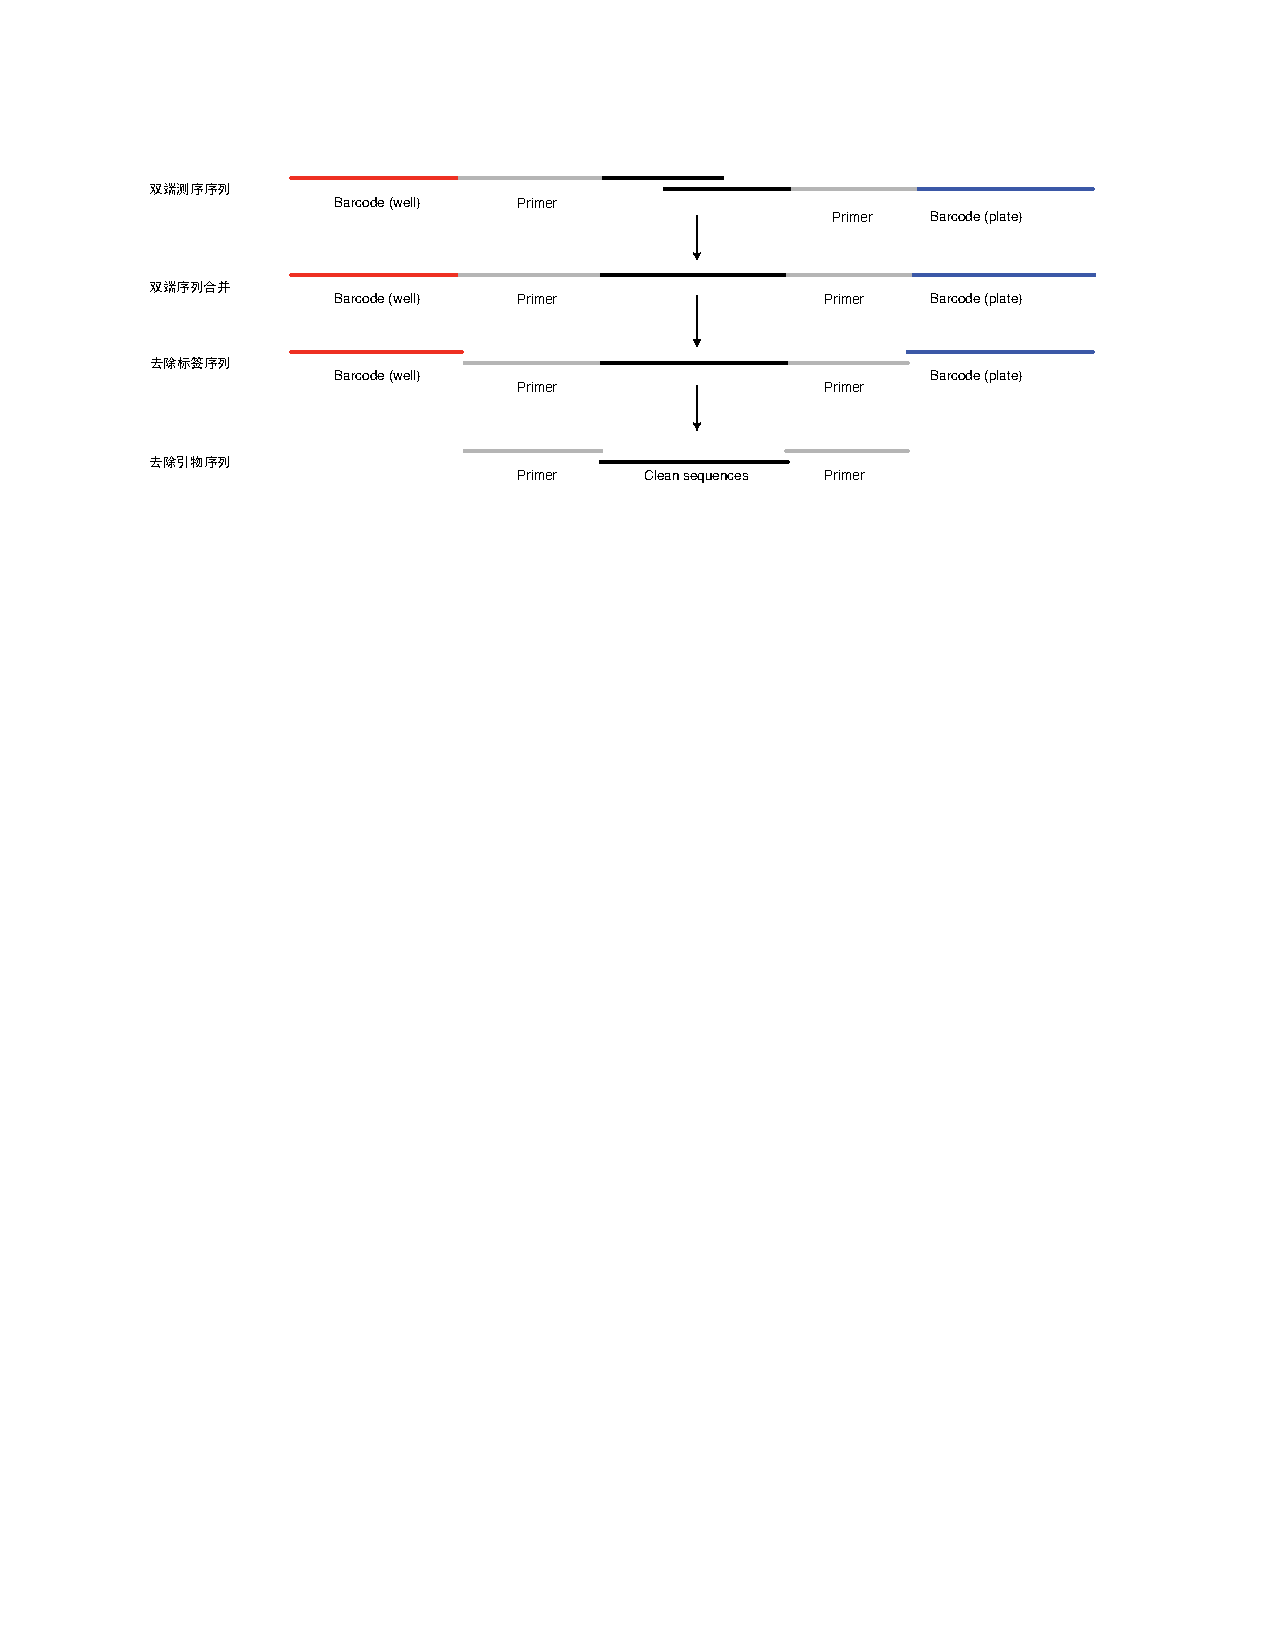
\includegraphics[width=0.98\textwidth]{img/数据预处理.pdf}
			\caption{数据预处理流程}
		\end{figure}
	\end{frame}

	\begin{frame}{微生物物种鉴定与功能预测}{物种鉴定}
		\begin{enumerate}
			\item 去除重复序列,获得序列丰度
			\item 降噪(UNOISE 算法)鉴定 ASV,从头($de~novo$)去除嵌合体
			\item 构建 ASV 表并基于 RDP 数据库进行物种注释
		\end{enumerate}

		\begin{figure}
			\centering
			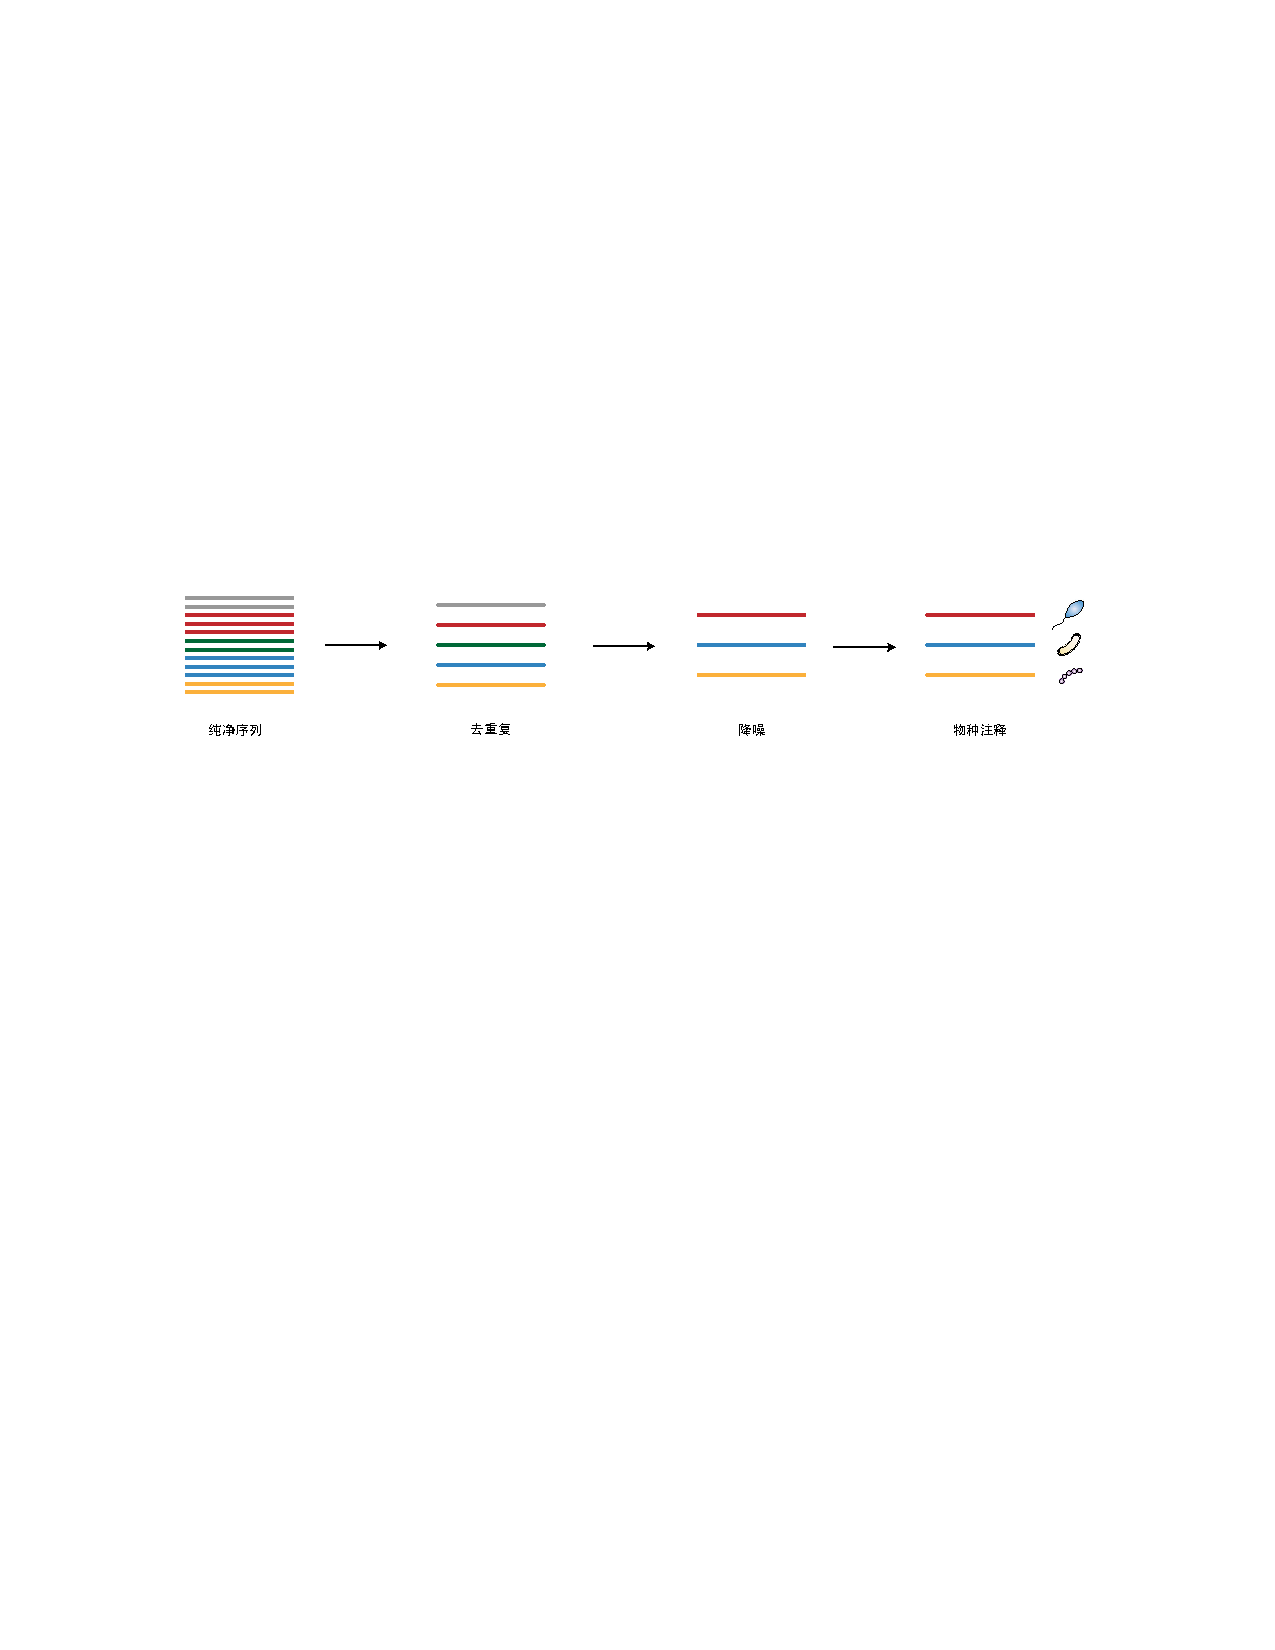
\includegraphics[width=\textwidth]{img/分析流程.pdf}
		\end{figure}
	\end{frame}

	\begin{frame}{微生物物种鉴定与功能预测}{挑选代表性序列}
		\begin{columns}
			\column{0.5\textwidth}
			\begin{itemize}
				\item ASV {\tiny (Amplicon Sequence Variants)} \\ \qquad ASV 则在 100\% 相似水平进行聚类,精度更高,结合降噪算法去除噪声序列所以在增加样本时,结果具有一致性。
			\end{itemize}
			
			\column{0.5\textwidth}
			\begin{itemize}
				\item OTU {\tiny (Operational Taxonomic Units)} \\ \qquad OTU 是一种聚类方式,通常在 97\% 的相似水平下聚类生成 OTU,选择每个聚类群中最高丰度序列作为代表性序列。
			\end{itemize}
		\end{columns}

		\begin{figure}
			\centering
			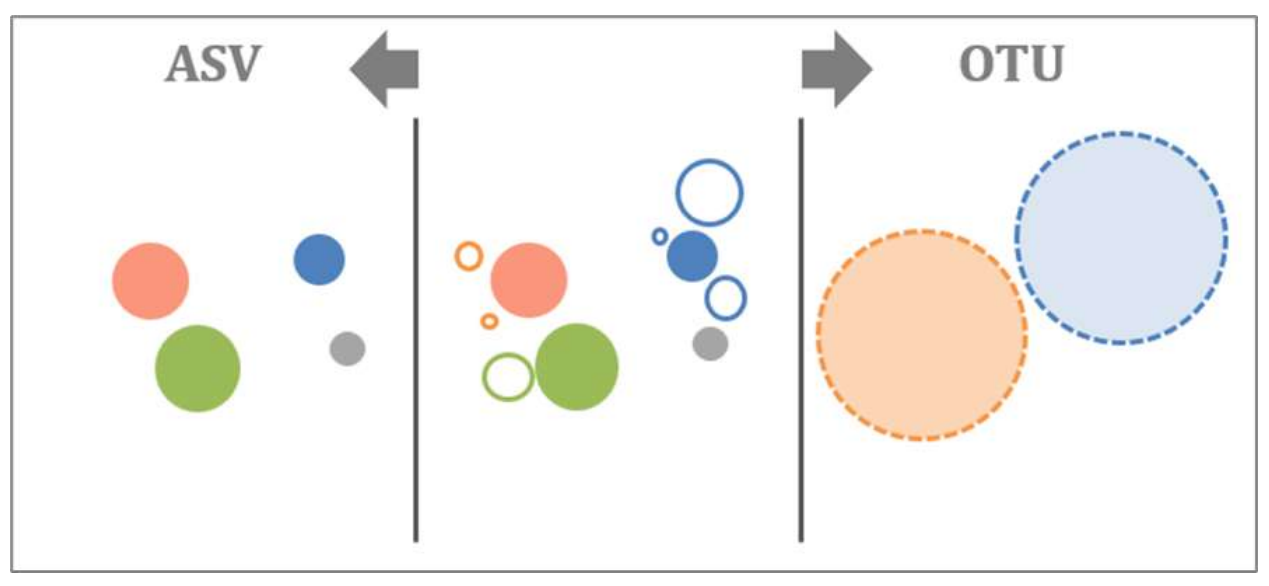
\includegraphics[width=0.7\textwidth]{img/OTUvsASV.png}
		\end{figure}
	\end{frame}

	\begin{frame}{微生物物种鉴定与功能预测}{物种注释}
		\qquad 基于 RDP 数据库进行物种注释,构建 ASV 表。

		\begin{figure}
			\centering
			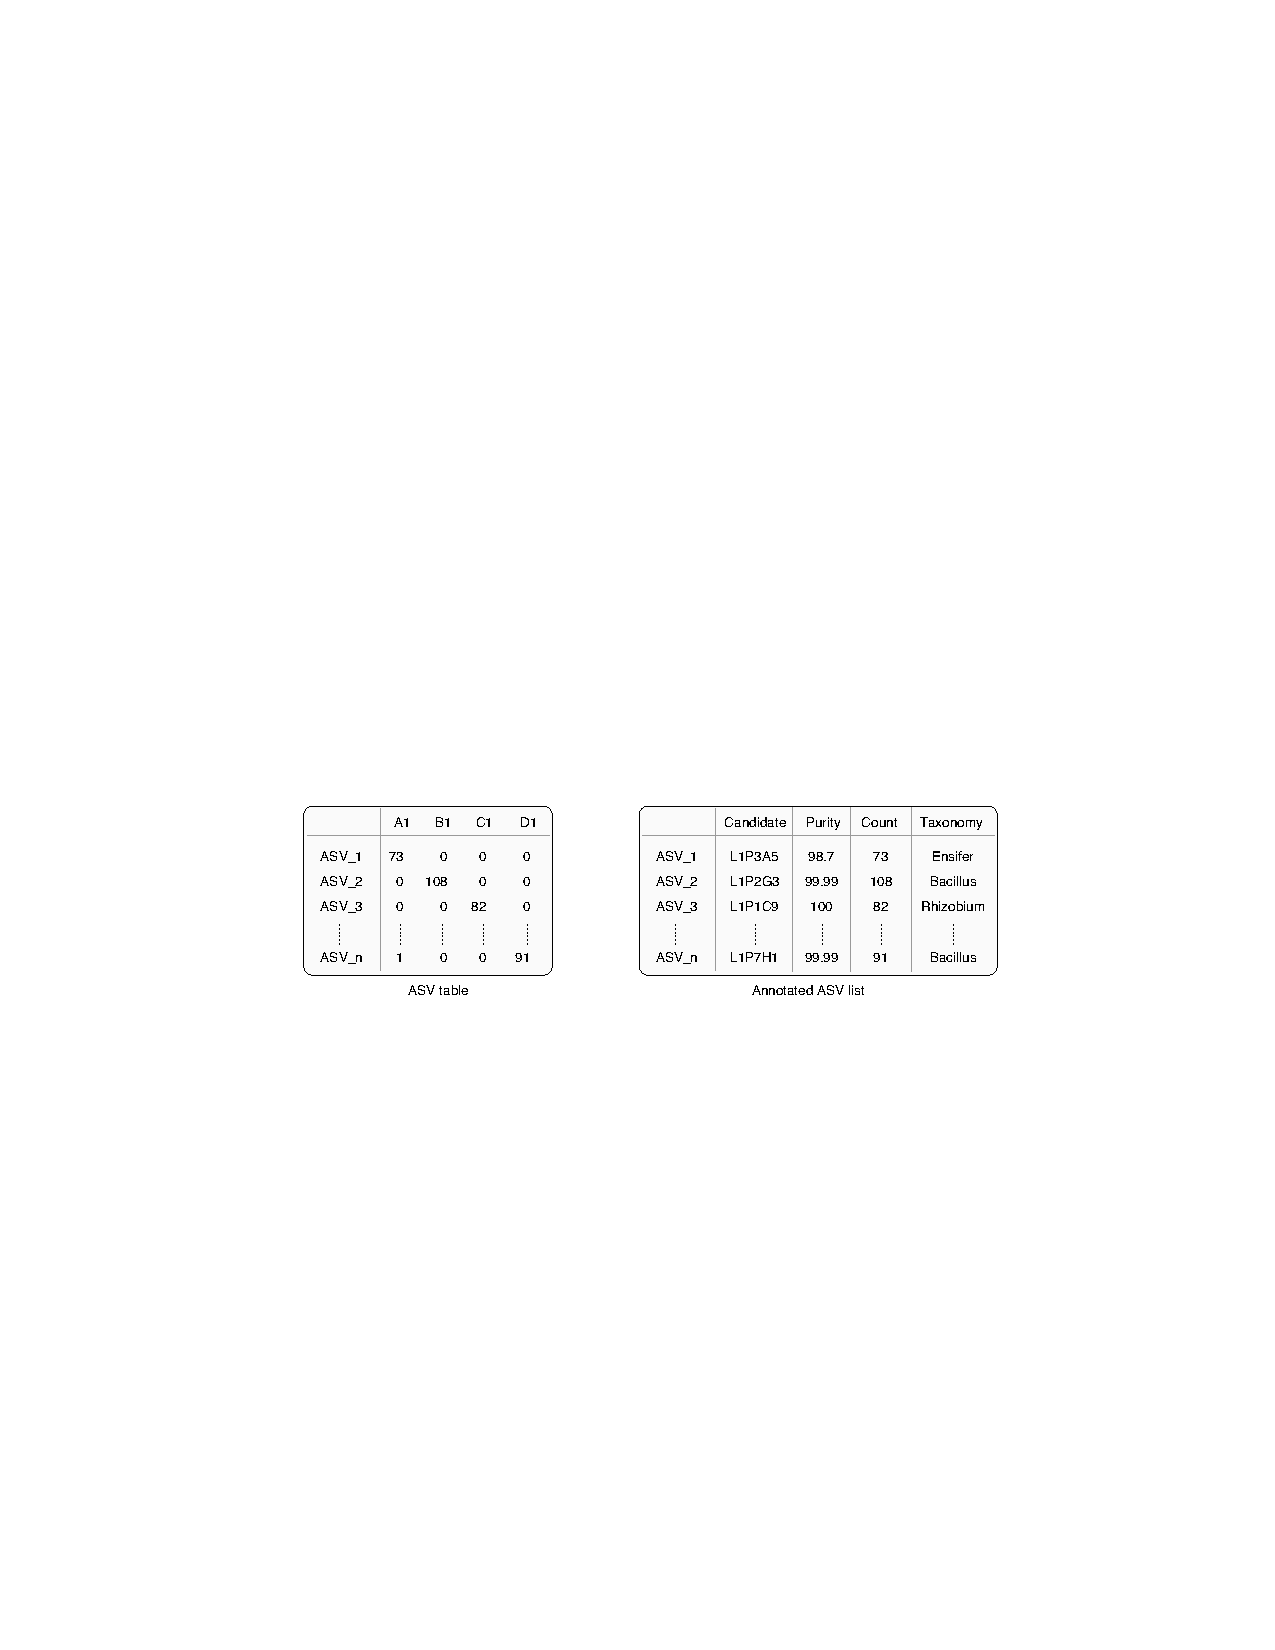
\includegraphics[width=\textwidth]{img/ASVtable.pdf}
		\end{figure}

	\end{frame}

	\begin{frame}{微生物物种鉴定与功能预测}{功能预测}
		\qquad 使用 PICRUSt2 进行功能预测(ASV 序列、丰度文件作为输入),预测基于多个基因家族数据库(KEGG同源基因、KO直系同源物、EC酶分类编号)。结果使用 R 包 ggpicrust2 进行可视化。
		\begin{figure}
			\centering
			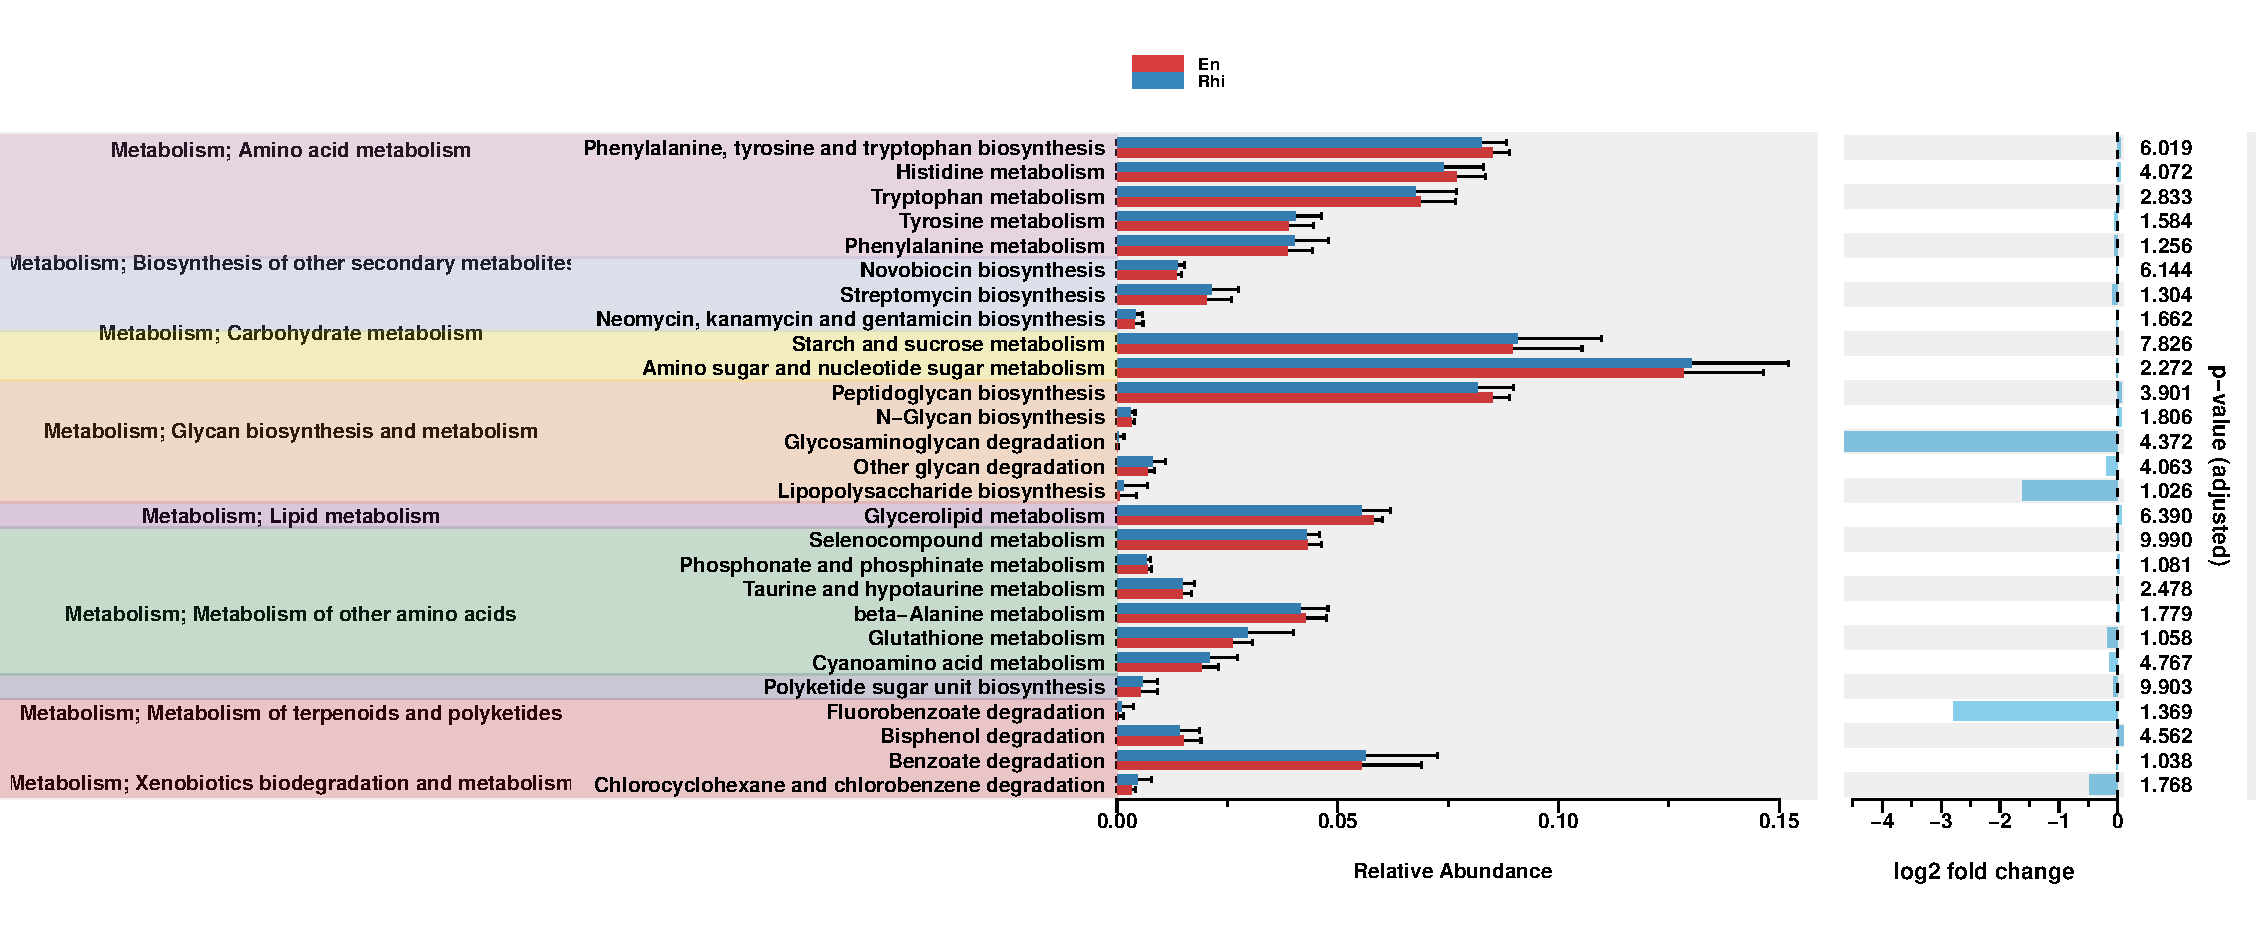
\includegraphics[width=0.9\textwidth]{img/RelativeAbundance60.pdf}
			\caption{基因功能预测部分结果}
		\end{figure}
	\end{frame}

	\begin{frame}{微生物物种鉴定与功能预测}{部分可视化结果}
		\begin{figure}
			\subfigure[根内菌种]{
				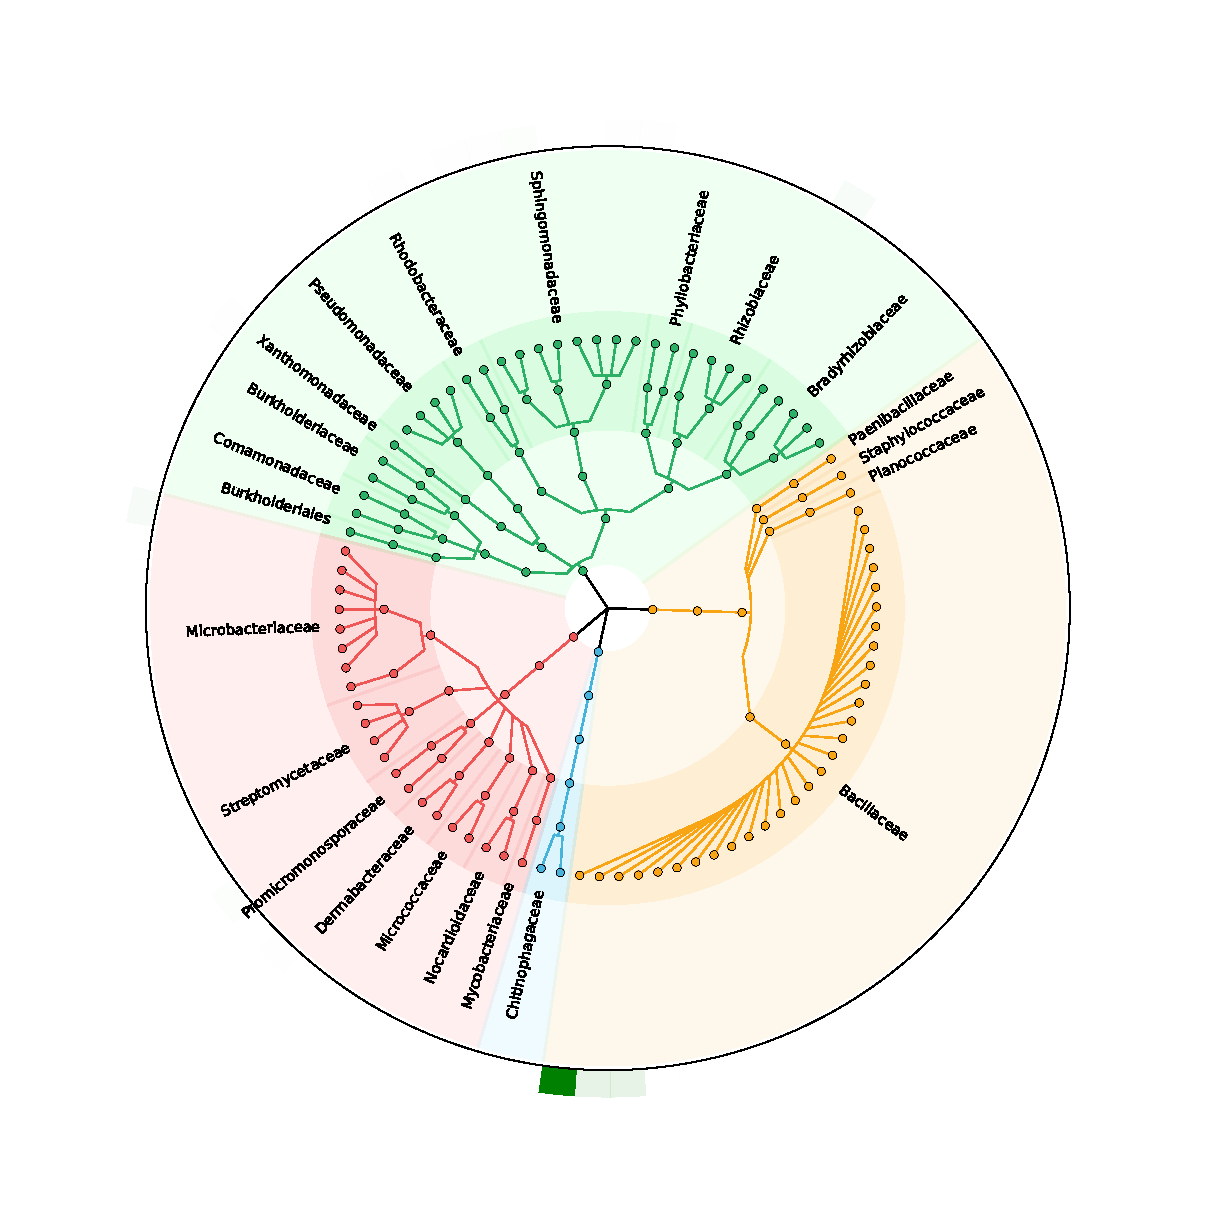
\includegraphics[width=0.45\textwidth]{img/en_graphlan.pdf}
				}
				\subfigure[根内、根际微生物功能差异]{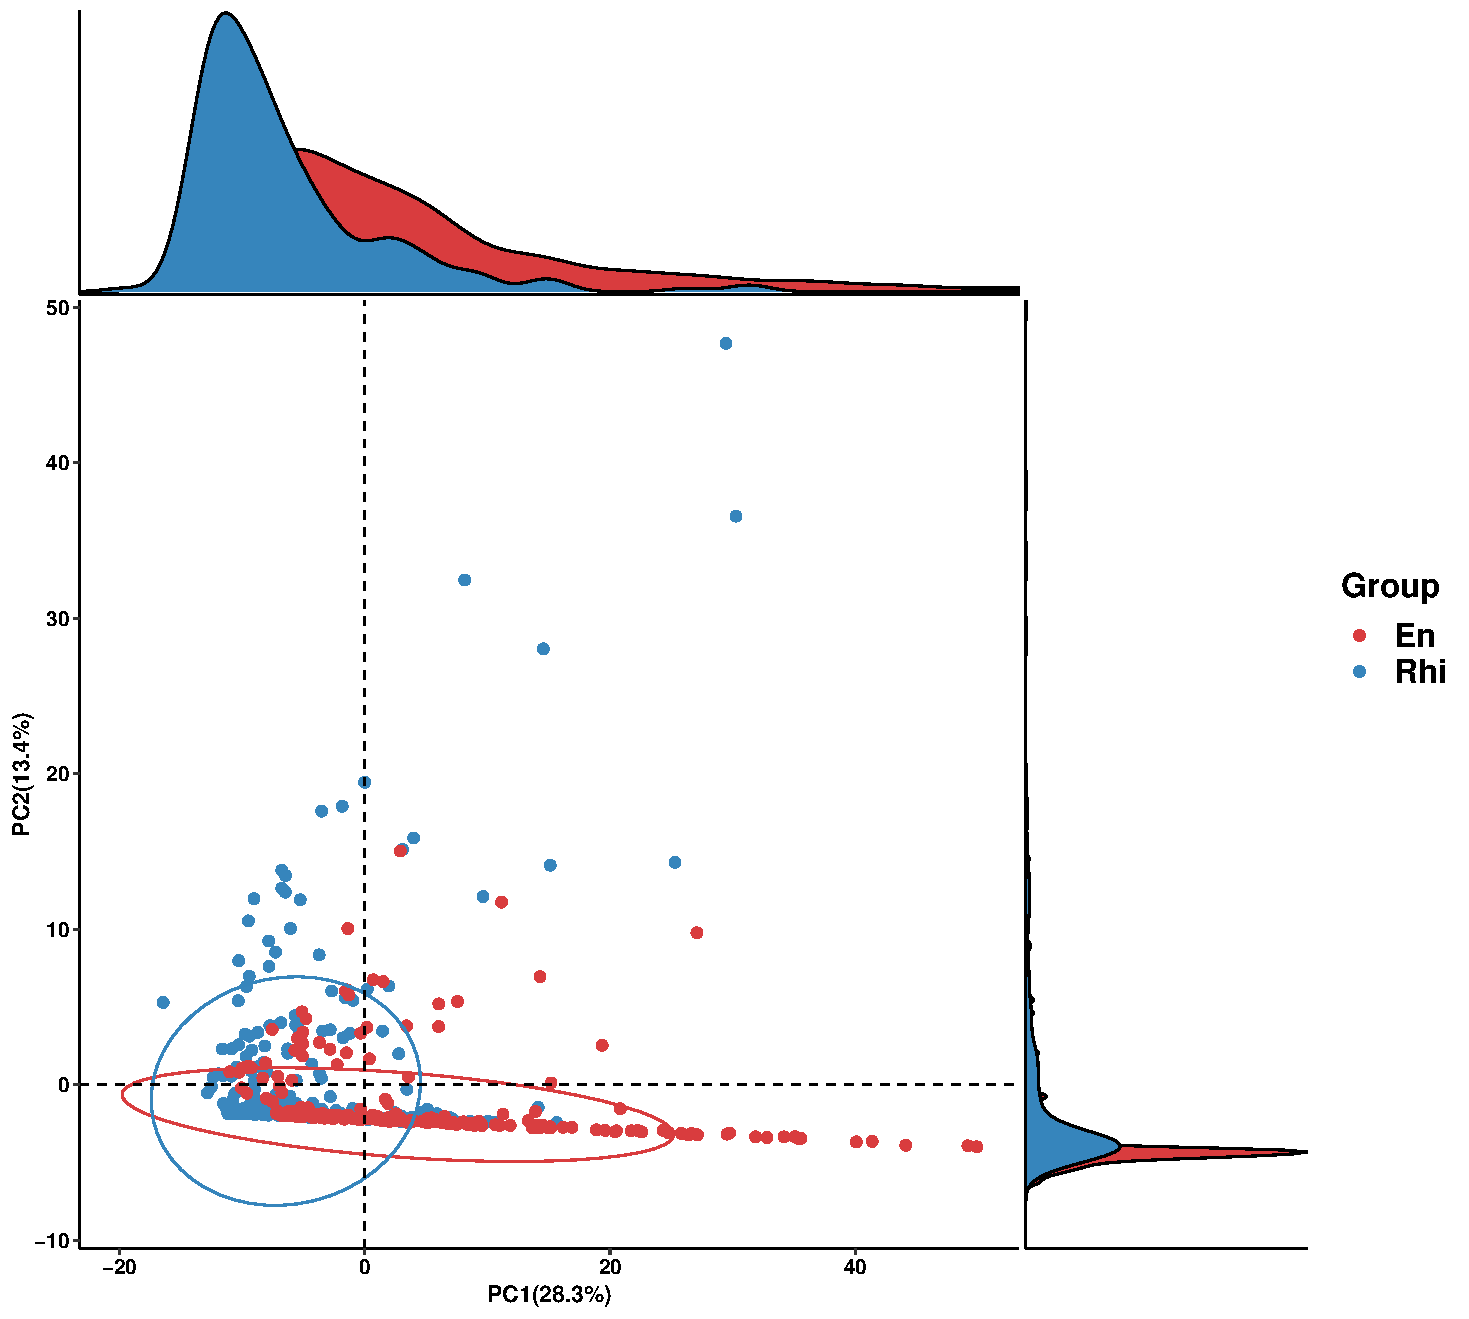
\includegraphics[width=0.5\textwidth]{img/PCA_KO.pdf}}
		\end{figure}
	\end{frame}

	\subsection{线虫 ChIP-Seq 数据分析}
	\begin{frame}{线虫 ChIP-Seq 数据分析}{流程}
		\begin{enumerate}
			\item FastQC 质控
			\item Trimmomatic 去除 adapter 序列
			\item BWA/Bowtie 建立参考基因组索引并比对
			\item Samtools 统计比对结果
			\item Peak Calling
			\item Motif 分析
			\item Peak 注释
			\item Geno Ontology
		\end{enumerate}
	\end{frame}

	\begin{frame}{线虫 ChIP-Seq 数据分析}{涉及软件}
		\begin{columns}
			\column{0.5\textwidth}
			\begin{itemize}
				\item FastQC
				\item Trimmomatic
				\item BWA
				\item Bowtie
				\item Samtools
			\end{itemize}
			
			\column{0.5\textwidth}
			\begin{itemize}
				\item Bedtools
				\item MACS
				\item MEME
				\item ChIPseeker
				\item PANTHER
			\end{itemize}
		\end{columns}
	\end{frame}
	
\begin{frame}{线虫 ChIP-Seq 数据分析}{部分结果}
	\begin{figure}[h]
		\begin{minipage}{0.45\linewidth}
			\centerline{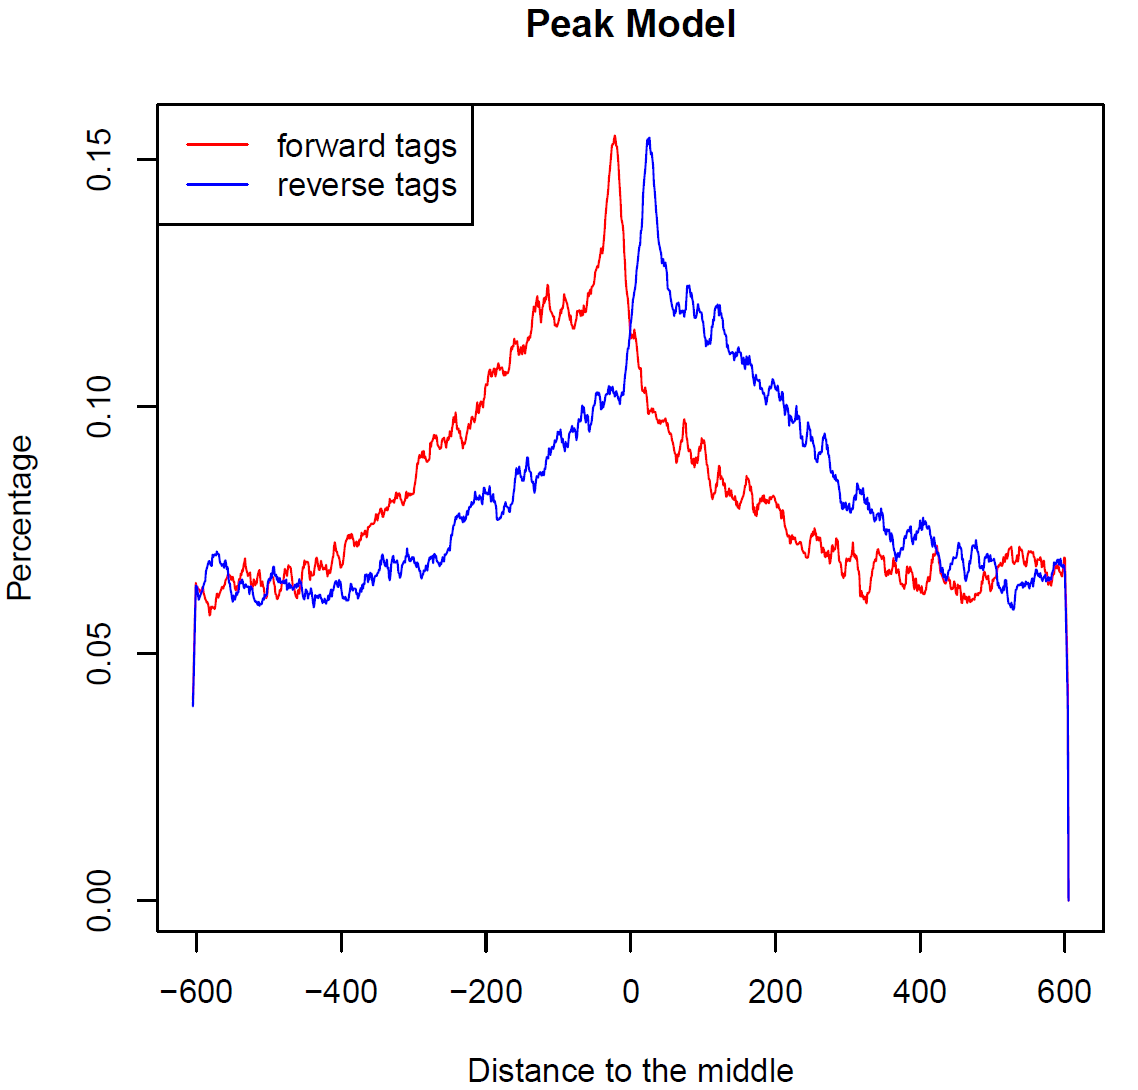
\includegraphics[width=\textwidth]{img/peak_model.png}}
		\end{minipage}
		\begin{minipage}{0.45\linewidth}
			\centerline{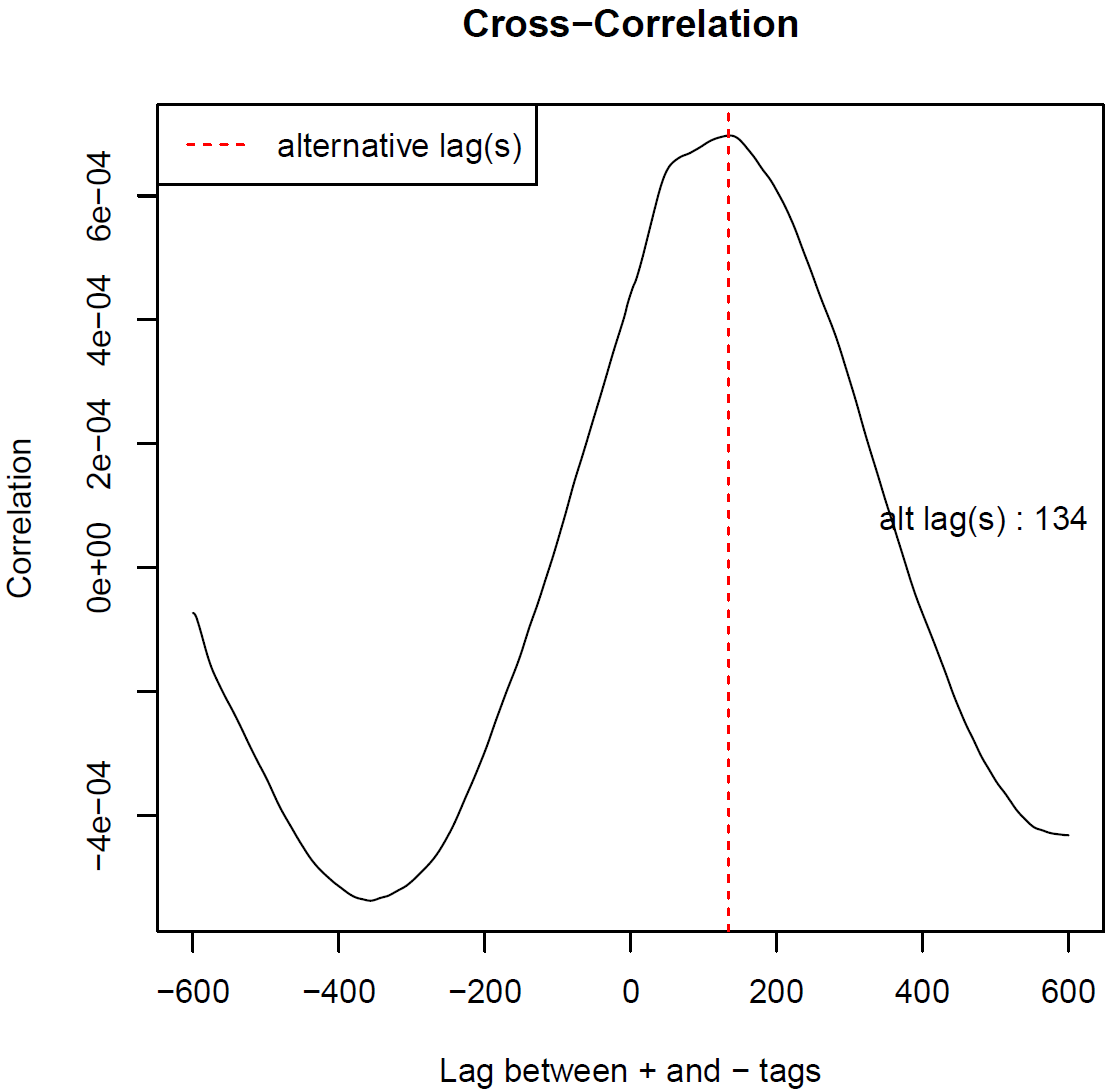
\includegraphics[width=\textwidth]{img/cross_correlation.png}}
	\end{minipage}
	
	\caption{Peak calling 结果}
	\end{figure}
\end{frame}

\begin{frame}{线虫 ChIP-Seq 数据分析}{部分结果}
	\begin{figure}
		\centering
		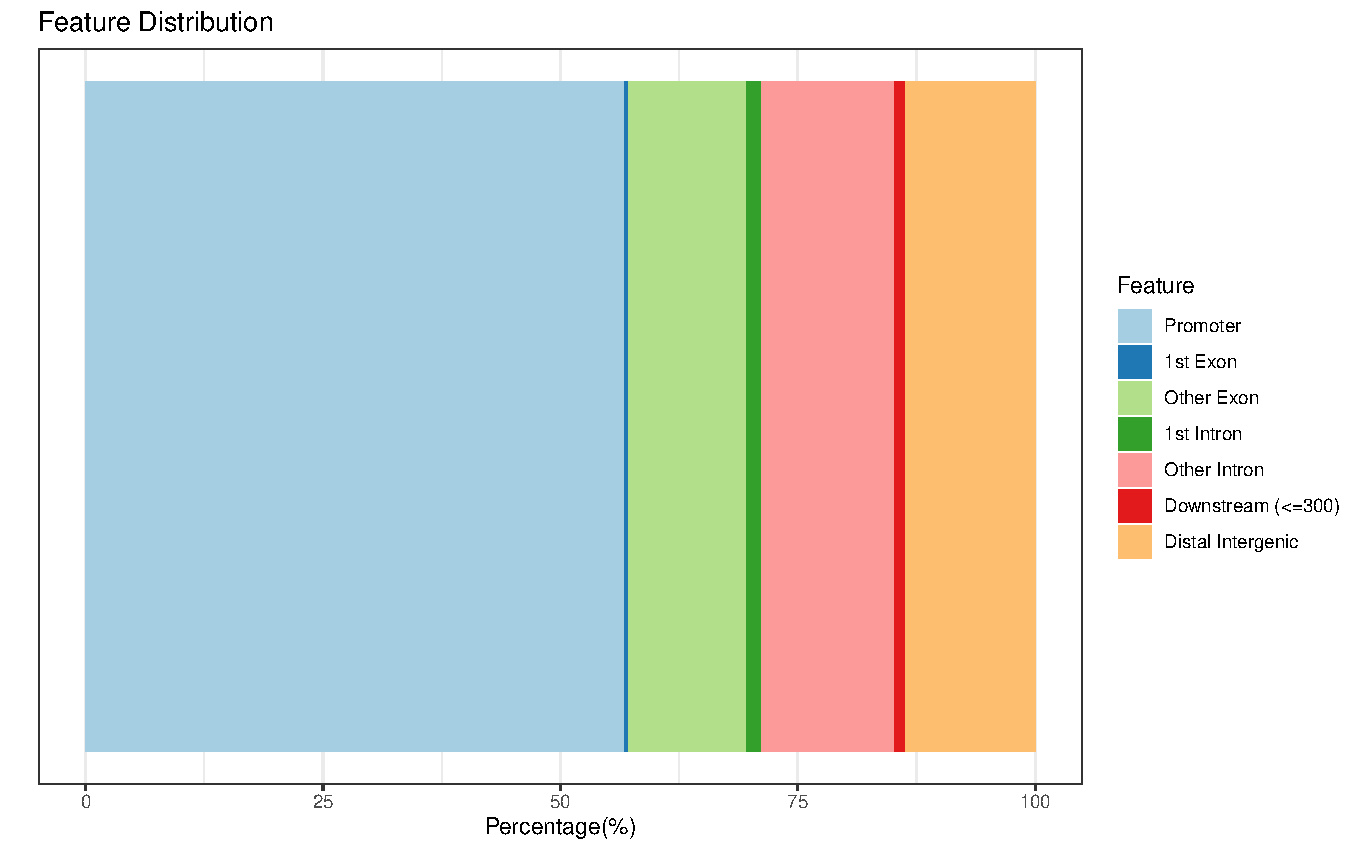
\includegraphics[width=0.9\textwidth]{img/peaks_feature_distribution.pdf}
	\end{figure}
\end{frame}

\subsection{枯草芽孢杆菌群比较基因组分析}
\begin{frame}{枯草芽孢杆菌群比较基因组分析}{分析流程}
	\begin{enumerate}
		\item 基因组组分分析
		\begin{itemize}
			\item Glimmer \& Prodigal
		\end{itemize}
		\item 基因功能分析
		\begin{itemize}
			\item GO Annotation
			\item COG Annotation
			\item KEGG Annotation
			\item CAZy Annotation
		\end{itemize}
		\item 泛基因组分析
		\begin{itemize}
			\item Core Gene
		\end{itemize}
		\item 比较基因组分析
			\begin{itemize}
				\item 系统发育树
				\item 共线性分析
			\end{itemize}
	\end{enumerate}
\end{frame}

	\section*{致谢}
	\begin{frame}
		\begin{center}
			\textcolor{myNewColorA}{\huge 谢谢!}
		\end{center}
	\end{frame}
	
\end{document}